%File: anonymous-submission-latex-2026.tex
\documentclass[letterpaper]{article} % DO NOT CHANGE THIS
\usepackage[submission]{aaai2026}  % DO NOT CHANGE THIS
\usepackage{times}  % DO NOT CHANGE THIS
\usepackage{helvet}  % DO NOT CHANGE THIS
\usepackage{courier}  % DO NOT CHANGE THIS
\usepackage[hyphens]{url}  % DO NOT CHANGE THIS
\usepackage{graphicx} % DO NOT CHANGE THIS
\urlstyle{rm} % DO NOT CHANGE THIS
\def\UrlFont{\rm}  % DO NOT CHANGE THIS
\usepackage{natbib}  % DO NOT CHANGE THIS AND DO NOT ADD ANY OPTIONS TO IT
\usepackage{caption} % DO NOT CHANGE THIS AND DO NOT ADD ANY OPTIONS TO IT
\frenchspacing  % DO NOT CHANGE THIS
\setlength{\pdfpagewidth}{8.5in} % DO NOT CHANGE THIS
\setlength{\pdfpageheight}{11in} % DO NOT CHANGE THIS
%
% These are recommended to typeset algorithms but not required. See the subsubsection on algorithms. Remove them if you don't have algorithms in your paper.
\usepackage{algorithm}
\usepackage{algorithmic}
\usepackage{amsmath}
\usepackage{amssymb}
\usepackage{bm}

%
% These are are recommended to typeset listings but not required. See the subsubsection on listing. Remove this block if you don't have listings in your paper.
\usepackage{newfloat}
\usepackage{listings}
\DeclareCaptionStyle{ruled}{labelfont=normalfont,labelsep=colon,strut=off} % DO NOT CHANGE THIS
\lstset{%
	basicstyle={\footnotesize\ttfamily},% footnotesize acceptable for monospace
	numbers=left,numberstyle=\footnotesize,xleftmargin=2em,% show line numbers, remove this entire line if you don't want the numbers.
	aboveskip=0pt,belowskip=0pt,%
	showstringspaces=false,tabsize=2,breaklines=true}
\floatstyle{ruled}
\newfloat{listing}{tb}{lst}{}
\floatname{listing}{Listing}
%
% Keep the \pdfinfo as shown here. There's no need
% for you to add the /Title and /Author tags.
\pdfinfo{
/TemplateVersion (2026.1)
}

% DISALLOWED PACKAGES
% \usepackage{authblk} -- This package is specifically forbidden
% \usepackage{balance} -- This package is specifically forbidden
% \usepackage{color (if used in text)
% \usepackage{CJK} -- This package is specifically forbidden
% \usepackage{float} -- This package is specifically forbidden
% \usepackage{flushend} -- This package is specifically forbidden
% \usepackage{fontenc} -- This package is specifically forbidden
% \usepackage{fullpage} -- This package is specifically forbidden
% \usepackage{geometry} -- This package is specifically forbidden
% \usepackage{grffile} -- This package is specifically forbidden
% \usepackage{hyperref} -- This package is specifically forbidden
% \usepackage{navigator} -- This package is specifically forbidden
% (or any other package that embeds links such as navigator or hyperref)
% \indentfirst} -- This package is specifically forbidden
% \layout} -- This package is specifically forbidden
% \multicol} -- This package is specifically forbidden
% \nameref} -- This package is specifically forbidden
% \usepackage{savetrees} -- This package is specifically forbidden
% \usepackage{setspace} -- This package is specifically forbidden
% \usepackage{stfloats} -- This package is specifically forbidden
% \usepackage{tabu} -- This package is specifically forbidden
% \usepackage{titlesec} -- This package is specifically forbidden
% \usepackage{tocbibind} -- This package is specifically forbidden
% \usepackage{ulem} -- This package is specifically forbidden
% \usepackage{wrapfig} -- This package is specifically forbidden
% DISALLOWED COMMANDS
% \nocopyright -- Your paper will not be published if you use this command
% \addtolength -- This command may not be used
% \balance -- This command may not be used
% \baselinestretch -- Your paper will not be published if you use this command
% \clearpage -- No page breaks of any kind may be used for the final version of your paper
% \columnsep -- This command may not be used
% \newpage -- No page breaks of any kind may be used for the final version of your paper
% \pagebreak -- No page breaks of any kind may be used for the final version of your paperr
% \pagestyle -- This command may not be used
% \tiny -- This is not an acceptable font size.
% \vspace{- -- No negative value may be used in proximity of a caption, figure, table, section, subsection, subsubsection, or reference
% \vskip{- -- No negative value may be used to alter spacing above or below a caption, figure, table, section, subsection, subsubsection, or reference

\setcounter{secnumdepth}{1} %May be changed to 1 or 2 if section numbers are desired.

% Custom macros
\newcommand{\bxi}{\boldsymbol{\xi}}
\newcommand{\bx}{\bm{x}}
\newcommand{\avg}[1]{\langle #1 \rangle}
\newcommand{\e}{{\mathrm{e}}}
\newcommand{\dd}{{\mathrm{d}}}
% \newcommand{\Bnet}{\beta_{\mathrm{net}}}
\newcommand{\Bnet}{\beta}
\newcommand{\phieq}{\varphi_{\mathrm{eq}}}
\newcommand{\fret}{f_{\mathrm{ret}}}
\newcommand{\gmax}{g_{\max}}
\newcommand{\acGauss}{\alpha_c^{\mathrm{G}}}
\newcommand{\ac}{\alpha_c}
\newcommand{\acBd}{\alpha_c^{\mathrm{bd}}}
\newcommand{\acSd}{\alpha_c^{\mathrm{sd}}}
\newcommand{\acSp}{\alpha_c^{\mathrm{sp}}}
\newcommand{\p}{\partial}
\newcommand{\cas}{\textstyle\frac}


% The file aaai2026.sty is the style file for AAAI Press
% proceedings, working notes, and technical reports.
%

% Title

% Your title must be in mixed case, not sentence case.
% That means all verbs (including short verbs like be, is, using,and go),
% nouns, adverbs, adjectives should be capitalized, including both words in hyphenated terms, while
% articles, conjunctions, and prepositions are lower case unless they
% directly follow a colon or long dash
\title{\bfseries Thermodynamic approach and Saddle-Dominated Capacity
of the LSE Dense Associative Memory}

\author{
    %Authors
    % All authors must be in the same font size and format.
    Written by AAAI Press Staff\textsuperscript{\rm 1}\thanks{With help from the AAAI Publications Committee.}\\
    AAAI Style Contributions by Pater Patel Schneider,
    Sunil Issar,\\
    J. Scott Penberthy,
    George Ferguson,
    Hans Guesgen,
    Francisco Cruz\equalcontrib,
    Marc Pujol-Gonzalez\equalcontrib
}
\affiliations{
    %Afiliations
    \textsuperscript{\rm 1}Association for the Advancement of Artificial Intelligence\\
    % If you have multiple authors and multiple affiliations
    % use superscripts in text and roman font to identify them.
    % For example,

    % Sunil Issar\textsuperscript{\rm 2},
    % J. Scott Penberthy\textsuperscript{\rm 3},
    % George Ferguson\textsuperscript{\rm 4},
    % Hans Guesgen\textsuperscript{\rm 5}
    % Note that the comma should be placed after the superscript

    1101 Pennsylvania Ave, NW Suite 300\\
    Washington, DC 20004 USA\\
    % email address must be in roman text type, not monospace or sans serif
    proceedings-questions@aaai.org
%
% See more examples next
}

%Example, Single Author, ->> remove \iffalse,\fi and place them surrounding AAAI title to use it
\iffalse
\title{My Publication Title --- Single Author}
\author {
    Author Name
}
\affiliations{
    Affiliation\\
    Affiliation Line 2\\
    name@example.com
}
\fi

\iffalse
%Example, Multiple Authors, ->> remove \iffalse,\fi and place them surrounding AAAI title to use it
\title{My Publication Title --- Multiple Authors}
\author {
    % Authors
    First Author Name\textsuperscript{\rm 1},
    Second Author Name\textsuperscript{\rm 2},
    Third Author Name\textsuperscript{\rm 1}
}
\affiliations {
    % Affiliations
    \textsuperscript{\rm 1}Affiliation 1\\
    \textsuperscript{\rm 2}Affiliation 2\\
    firstAuthor@affiliation1.com, secondAuthor@affilation2.com, thirdAuthor@affiliation1.com
}
\fi


% REMOVE THIS: bibentry
% This is only needed to show inline citations in the guidelines document. You should not need it and can safely delete it.
\usepackage{bibentry}
% END REMOVE bibentry

\begin{document}

\maketitle

\begin{abstract}
The Dense Associative Memory with log-sum-exp (LSE) kernel on the $N$-sphere
stores $M = \exp(\alpha N)$ patterns at load $\alpha$. A Gaussian approximation
of the inter-pattern alignments gives a zero-temperature capacity
$\alpha_c = 1/2$, independent of the kernel sharpness $\Bnet$, the
Gaussian-ensemble threshold of \citet{lucibello2024exponential}. Using the exact
spherical alignment density, we build a finite-temperature theory of retrieval.
The sum over non-target patterns is then set by an interior saddle rather than by
the right tail of the Gaussian, which restores the $\Bnet$-dependence: at $T = 0$
the capacity grows from $\sim\Bnet$ at small $\Bnet$ to $\tfrac12 \ln\Bnet$ at
large $\Bnet$, is $\approx 0.6226$ at $\Bnet = 1$, and reproduces the exact
spherical threshold of \citeauthor{lucibello2024exponential}. At $T > 0$ the retrieval
basin is bounded by a single-pattern spinodal, beyond which it no longer exists;
below it the basin is metastable, with a Kramers escape time exponential in $N$.
We confirm the resulting $(\alpha, T)$ stability diagram by Monte Carlo: the
Full sampler stores all $M$ patterns but reaches only $N \sim 25$, the Cone
sampler that keeps only the patterns in a cone around the target reaches
$N \sim 30$, and a pattern-free Bulk sampler that follows the leading-order
free-energy profile reaches $N \sim 10^4$. All three agree with the predicted
spinodal to within the residual finite-$N$ gap.
\end{abstract}



% Uncomment the following to link to your code, datasets, an extended version or similar.
% You must keep this block between (not within) the abstract and the main body of the paper.
% \begin{links}
%     \link{Code}{https://aaai.org/example/code}
%     \link{Datasets}{https://aaai.org/example/datasets}
%     \link{Extended version}{https://aaai.org/example/extended-version}
% \end{links}


% ----------------------------------------------------------------------------------
% ----------------------------------------------------------------------------------
% ----------------------------------------------------------------------------------

\section{Introduction}

Modern dense associative memory (DAM) models begin with \citet{krotov2016dense},
who generalized the classical Hopfield network~\citep{Hopfield1982} from pairwise
to polynomial interactions, raising the storage capacity from linear to
polynomial in the number of neurons $N$ while preserving the ability to
retrieve previously stored information from noisy or corrupted input data. 
Taking the polynomial degree to infinity yields an exponential capacity~\citep{demircigil2017model}:
for binary neurons (state space $\{-1,+1\}^{N}$), the limiting capacity is
$M_{\rm c} = \exp(\alpha_{\rm c} N)$ with load $\alpha_{\rm c} = (\ln 2)/2 \approx 0.35$.

The same exponential scaling carries over to continuous states.
\citet{ramsauer2021hopfield} introduced a modern Hopfield network whose state is
a continuous vector in $\mathbb{R}^N$ and whose energy is a log-sum-exp (LSE) of the state-pattern
alignments. We take both the stored patterns $\bxi^\mu$ and the retrieval state
$\bx$ on the sphere $|\bx|^2 = N$, and store $M = \exp(\alpha N)$ patterns at load $\alpha$. 
The energy then reads
\begin{equation}
H(\bx) = -\Bnet^{-1}\ln\sum_{\mu=1}^{M}\exp\!\big[-\Bnet\,N (1-\phi^\mu) \big],
\label{eq:lse}
\end{equation}
where $\Bnet$ is a kernel sharpness controlling how strongly the energy
distinguishes patterns, and $\phi^\mu$ is the \textit{alignment} of the current state $\bx$ 
with the $\mu$-th pattern $\bxi^\mu$,
\begin{equation}
    \phi^\mu(\bm{x}) = N^{-1} \bm{x} \cdot \bm{\xi}^\mu\,.
    \label{eq:alignment}
\end{equation}

All these models are energy-based. What sets the LSE energy apart from 
the classical, polynomial, and exponential models is the logarithm: 
it acts as a smooth maximum, keeping the energy extensive in $N$
rather than exponentially large, while its gradient is a softmax over patterns,
so the retrieval update replaces the state by a softmax-weighted average of the
stored patterns, exactly like the attention mechanism of transformers.
Model~\eqref{eq:lse} is the Gaussian-kernel member of a family of kernel-based
energies. Replacing the Gaussian by the compactly
supported Epanechnikov kernel gives the log-sum-ReLU (LSR)
model~\citep{hoover2025dense}.

A natural question is how retrieval survives thermal noise. At a finite
temperature $T$ of the thermal bath (distinct from the kernel sharpness $\Bnet$), the boundary
$\alpha_c(\Bnet, T)$ in the load-temperature plane separates cues that relax back
to their target from cues that escape to spurious states.
\citet{icml2026theory} derived this boundary for the LSE and LSR kernels under a
Gaussian approximation of the inter-pattern alignment density, obtaining for LSE
a $\Bnet$-independent zero-temperature load $\alpha_c = 1/2$, and identifying the 
Gaussian approximation as the source of error. Brute-force Monte
Carlo~\citep{iclr2026mc} then showed deviations from the Gaussian
prediction, with the retrieval region extending to larger $\alpha$ as $T\to0$.

Here we revisit the LSE capacity on the $N$-sphere using the exact spherical
alignment density, both analytically and by Monte Carlo, across the full
$(\alpha, T)$ plane. The sum over non-target patterns is governed by an interior
saddle of the partition-sum integrand rather than by the right edge of the
alignment distribution, which restores the $\Bnet$-dependence missing from the
Gaussian estimate. At $T = 0$ the resulting capacity reproduces the exact
spherical threshold of \citet{lucibello2024exponential} and lies above the
rigorous storage lower bound of \citet{ramsauer2021hopfield}. At $T > 0$ the
retrieval well is bounded by a spinodal, the limit of metastability beyond which
the well disappears; below it the well persists metastably, and a trapped cue
escapes only over a barrier, with a lifetime exponential in $N$, a Kramers escape
\citep{kramers1940, hanggi1990}. This resolves the low-$T$ deviations seen in
simulations.

The paper is organized as follows. Section \ref{sec:theory} builds the
finite-temperature retrieval theory from the exact spherical alignment density:
the Gaussian baseline and why it fails, the interior saddle that fixes the noise
floor, the zero-temperature capacity, and the finite-temperature spinodal. The
Monte Carlo schemes section \ref{sec:mc} describes the Full, Cone, and Bulk samplers. The
Results section presents the stability diagram in the $(\alpha, T)$ plane at
$\Bnet = 1$, compares it against the Gaussian and spinodal predictions, and
examines the finite-$N$ behavior. The Discussion section \ref{sec:discussion} collects the
implications and the relation to the literature.


% ----------------------------------------------------------------------------------
% ----------------------------------------------------------------------------------
% ----------------------------------------------------------------------------------

\section{Retrieval at large $N$}
\label{sec:theory}

Let the retrieval pattern $\bxi^1$ and a spurious pattern $\bxi$ be drawn independently
and uniformly from the sphere of radius $\sqrt N$ in $\mathbb{R}^N$. The alignment
\begin{equation}
    \varphi(\bxi) \equiv N^{-1} \bxi^1\cdot\bxi
\end{equation}
is the cosine of the angle between them. By rotational symmetry we may fix the first pattern
along the coordinate axis $\bm e_1$ and treat the spurious pattern as a unit vector $\bm u$
uniformly distributed on $S^{N-1}$.
The alignment is its first coordinate, $\varphi=u_1$, and we seek the density of
$u_1$ induced by the uniform measure on the sphere.
The probability that $u_1$ lies in $[\varphi,\varphi+\dd\varphi]$ equals the area of the corresponding 
spherical band divided by the total area of $S^{N-1}$. Decomposing $\bm u=(u_1,\bm u_\perp)$, 
the constraint $|\bm u|=1$ fixes $|\bm u_\perp|=\sqrt{1-\varphi^2}$, so the points at height 
$\varphi$ form a sphere $S^{N-2}$ of radius $\sqrt{1-\varphi^2}$, with surface area
$\propto (1-\varphi^2)^{(N-2)/2}$. The band thickness is $\dd\varphi/\sqrt{1-\varphi^2}$, 
since the surface is inclined with respect to the axis. Normalizing the band area
$\propto(1-\varphi^2)^{(N-3)/2}\dd\varphi$ gives the density
\begin{equation}
h(\varphi)=C_N(1-\varphi^2)^{(N-3)/2}
\label{eq:exact_density}
\end{equation}
with the normalization constant
\begin{equation}
C_N=\frac{\Gamma(N/2)}{\sqrt\pi\;\Gamma\!\big((N-1)/2\big)}\,.
\end{equation}

The density is symmetric about $\varphi=0$, with mean zero and variance $1/N$. As $N\to\infty$ it 
concentrates near the equator and approaches a Gaussian,
\begin{equation}
    h(\varphi)\;\longrightarrow \;\sqrt{\tfrac{N}{2\pi}} \; \e^{-N\varphi^2/2}\,,
    \label{eq:gaussian} 
\end{equation}
so distinct high-dimensional patterns are nearly orthogonal: typical alignments are of order $N^{-1/2}$. 
The exact law is retained where the rare large-alignment tail matters;
the Gaussian form matches only near the center.
The density~\eqref{eq:exact_density} and its Gaussian limit are the spherical
and Gaussian rate functions of \citet{lucibello2024exponential}.

\paragraph{Extreme-value attempts.}
The exact density~\eqref{eq:exact_density} and its Gaussian
limit~\eqref{eq:gaussian} agree near $\varphi = 0$ but differ at
the edge: $(1-\varphi^2)^{(N-3)/2}$ vanishes at $\varphi = \pm 1$
since two distinct points on the sphere cannot align perfectly,
while the Gaussian keeps a heavier tail there, of order $\e^{-N/2}$.
This single difference controls the extreme of
$M = \e^{\alpha N}$ alignments and, through it, the capacity bound
of~\citet{ramsauer2021hopfield}.

\citeauthor{ramsauer2021hopfield}'s Theorem~4 ties retrieval to the
separation of a target pattern from its nearest neighbour,
$N(1-\varphi_{\max})$, with $\varphi_{\max}$ the highest alignment
among the $M$ patterns: capacity is reached when a competing pattern
approaches the target, $\varphi_{\max} \to 1$.  Their Theorem~3 makes
this quantitative.  The softmax sum
$S(\bm x)$ from~\eqref{eq:lse}, at the target
$\bm x = \bxi^1$, splits as
\begin{align}
S(\bxi^1) &= 1 + S_{\rm spur},
\label{eq:softmax_sum}\\
S_{\rm spur} &= \sum_{\mu=2}^{M}\exp\!\big[\Bnet N(\varphi^{1\mu} - 1)\big],
\label{eq:spur_sum}
\end{align}
and replacing $S_{\rm spur}$ by $M$ times its largest term gives
\begin{equation}
S_{\rm spur} \;\le\; M\,\e^{-\Bnet N(1-\varphi_{\max})}
   \;=\; \e^{N(\alpha - \Bnet(1-\varphi_{\max}))}.
\label{eq:ramsauer_bound}
\end{equation}
$S_{\rm spur}$ overtakes the retrieval term once
$\varphi_{\max} > 1 - \alpha/\Bnet$, so the capacity solves
$\varphi_{\max}(\alpha) = 1 - \alpha/\Bnet$, where
$\varphi_{\max}(\alpha)$ is the extreme of $M$ samples from $h$.
The notation map between \citeauthor{ramsauer2021hopfield} and this
paper, with literal page and equation references, is in
Appendix~\ref{sec:appendix_ramsauer}.

The two choices of density now give two capacities.  Under the exact
density, the extreme solves
\begin{equation}
\varphi_{\max} \;=\; \sqrt{1 - \e^{-2\alpha}} \;<\; 1 \quad\text{for every }\alpha,
\label{eq:varphi_max}
\end{equation}
and the capacity equation becomes
\begin{equation}
\sqrt{1 - \e^{-2\alpha}} \;=\; 1 - \frac{\alpha}{\Bnet},
\label{eq:ramsauer_capacity}
\end{equation}
finite and $\Bnet$-dependent.  This is the spherical-pattern
capacity $\alpha_c(\Bnet) = \alpha_1(\Bnet)$ derived rigorously in
the statistical-mechanics analysis of
\citet{lucibello2024exponential}.  Under the Gaussian
approximation, the heavier tail at $\varphi = 1$ lets
$\varphi_{\max}$ reach $1$ at the $\Bnet$-independent load
$\acGauss = 1/2$, recovering the Gaussian-density threshold of
\citet{icml2026theory} and the i.i.d.-Gaussian typical-pattern
threshold $\alpha_1(\lambda{=}1) = 1/2$ of
\citet{lucibello2024exponential}.

Neither result is tight.  The bound~\eqref{eq:ramsauer_bound}
replaces a sum of $M$ terms by $M$ times its largest, an
overestimate of $S_{\rm spur}$.  The saddle-point analysis below
evaluates $S_{\rm spur}$ without that approximation.

\paragraph{Saddle-point evaluation.}
The spurious patterns are i.i.d. uniform on the sphere and independent of $\bx$,
so for any $\bx$ with $|\bx|^2 = N$ the projections
$\varphi^\mu(\bx) = \bx \cdot \bxi^\mu / N$ have marginal
density~\eqref{eq:exact_density}. The spurious sum therefore has the same
distribution at every $\bx$ on the sphere; in particular at $\bx = \bxi^1$, where
the projections become the inter-pattern alignments $\varphi_{1\mu}$. With
$M = \e^{\alpha N}$, the sum concentrates around its expectation, and
\begin{equation}
    S_{\rm spur} \approx M \int_{-1}^{1} \dd\varphi\, h(\varphi) \exp[\Bnet N(\varphi - 1)].
    \label{eq:spur_integral}
\end{equation}
The large-$N$ limit of~\eqref{eq:spur_integral} is set by a saddle point. The
saddle $\varphi^*$ solves $\p g(\varphi, \Bnet)/\p\varphi = 0$, with
\begin{equation}
    g(\varphi, \Bnet) = \ln(1-\varphi^2)/2 + \Bnet\,\varphi\,.
\end{equation}
This gives the saddle point at
\begin{equation}
\varphi^*(\Bnet) = \frac{\sqrt{1+4\Bnet^2} - 1}{2\Bnet}\,,
\label{eq:saddle}
\end{equation}
and the saddle value
\begin{equation}
g_{\max}(\Bnet) = g(\varphi^*, \Bnet) = \frac12 \ln(1 - \varphi^{*\,2}) + \Bnet\,\varphi^*\,.
\label{eq:saddle_value}
\end{equation}
The leading-order spurious sum is then
\begin{equation}
    S_{\rm spur} \sim \exp[N(\alpha + g_{\max}(\Bnet) - \Bnet)]\,.
    \label{eq:spurious_saddle}
\end{equation}
Appendix~A derives the prefactor; it depends only on $\varphi^*(\Bnet)$ and equals
$1.082$ at $\Bnet = 1$. In the large-$N$ limit only the leading term in the
exponent (proportional to $N$) survives, so the prefactor is not needed at this
stage.

\paragraph{Zero-temperature capacity.}
The internal energy density $u = H/N$ from~\eqref{eq:lse} reads
\begin{equation}
    u(\varphi) = \begin{cases}
        1 - \varphi & \text{retrieval term dominates}, \\
        1 - [\alpha + g_{\max}(\Bnet)]/\Bnet & \text{spurious term dominates}.
    \end{cases}
    \label{eq:u_piecewise}
\end{equation}
The two branches meet in a cusp at
\begin{equation}
\varphi_c(\alpha, \Bnet) = (\alpha + g_{\max}(\Bnet))/\Bnet,
\label{eq:cusp}
\end{equation}
where dominance switches. At zero temperature the retrieval minimum sits at
$\varphi = 1$; it is the global minimum as long as $\varphi_c < 1$, giving the
zero-temperature capacity
\begin{equation}
\ac(\Bnet, 0) = \Bnet - g_{\max}(\Bnet).
\label{eq:capacity_T0}
\end{equation}
This boundary matches the exact spherical threshold of
\citet{lucibello2024exponential} at every $\Bnet$.

\paragraph{Geometric picture.}
Fig.~\ref{fig:varphi} summarises the different approaches at $\Bnet = 1$. The red
straight line is the cusp position $\varphi_c(\alpha)$; the saddle-point
capacity~\eqref{eq:capacity_T0} is the load at which it reaches $\varphi = 1$. The
blue solid curve is the exact-density extreme~\eqref{eq:varphi_max} (no finite
capacity); the blue dotted curve is its Gaussian approximation $\sqrt{2\alpha}$,
which gives the $\Bnet$-independent $\acGauss = 1/2$. The grey dashed line
$1 - \alpha/\Bnet$ is the \citeauthor{ramsauer2021hopfield}
condition~\eqref{eq:ramsauer_capacity}; its intersection with the blue solid curve
gives the \citeauthor{ramsauer2021hopfield} capacity, finite and $\Bnet$-dependent
but below the saddle-point capacity at every $\Bnet$.

\begin{figure}[t]
\centering
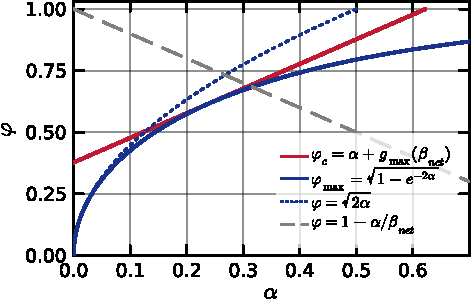
\includegraphics[width=0.45\textwidth]{panels_paper/cusp_vs_extreme.pdf}
\caption{Threshold curves at $\Bnet = 1$. Red straight line:
$\varphi_c(\alpha) = \alpha + g_{\max}(\Bnet)$, tangent to the blue solid curve at the
saddle $\varphi^*(\Bnet)$ (Appendix B). Blue solid:
the exact-density extreme alignment~\eqref{eq:varphi_max}.
Blue dotted: $\sqrt{2\alpha}$, its Gaussian approximation. Grey dashed:
$1 - \alpha/\Bnet$, the \citeauthor{ramsauer2021hopfield} condition.}
\label{fig:varphi}
\end{figure}

The red line is tangent to the blue solid curve at every $\Bnet$; as $\Bnet$
varies, the tangency point sweeps the entire blue solid curve. This follows from
the Legendre conjugacy between $g_{\max}(\Bnet)$ and $\varphi_{\max}(\alpha)$,
derived in Appendix~B. The geometric consequence is that the cusp
$\varphi_c(\alpha, \Bnet)$ lies above the maximum alignment $\varphi_{\max}(\alpha)$
at every $\alpha$: no individual spurious pattern enters the retrieval basin
$\varphi > \varphi_c$. Retrieval loss is therefore \textit{collective}, driven by
the bulk saddle of the spurious sum and not by any single spurious pattern
reaching the target. In the terminology of \citet{lucibello2024exponential}, the
retrieval boundary lies in the \textit{uncondensed} phase of the auxiliary REM,
where exponentially many patterns dominate the noise sum, as opposed to the
\textit{condensed} phase where a single pattern dominates.

\paragraph{Extension to finite temperature.}
At $T > 0$ the entropy density~\citep{icml2026theory}
\begin{equation}
    s(\varphi) = \tfrac{1}{2} \ln(1 - \varphi^2),
    \label{eq:entropy}
\end{equation}
adds to the internal energy, giving the free energy density
$f(\varphi) = u(\varphi) - T\,s(\varphi)$, plotted in Fig.~\ref{fig:cusp} for
$\alpha = 0.5$, $\Bnet = 1$ and several $T$. The profile has two minima: one at
$\varphi \approx 0$ from the spurious sum, one at $\varphi \approx 1$ from the
retrieval term. The retrieval minimum shifts from $\varphi = 1$ at $T = 0$ to
\begin{equation}
    \varphi_{\rm eq}(T) = \tfrac{1}{2}(\sqrt{T^2 + 4} - T)
    \label{eq:phi_eq}
\end{equation}
at $T > 0$, and disappears at the spinodal
$\varphi_{\rm eq}(T) = \varphi_c(\alpha, \Bnet)$, giving
\begin{equation}
    T_{\mathrm{sp}}(\alpha, \Bnet) \;=\; \frac{\Bnet^2 - (\alpha + \gmax(\Bnet))^2}
              {\Bnet\,(\alpha + \gmax(\Bnet))}\,.
    \label{eq:spinodal}
\end{equation}
Inverting~\eqref{eq:spinodal} at fixed $T$ gives the spinodal
capacity
\begin{equation}
    \ac(\Bnet, T) \;=\; \Bnet\,\varphi_{\rm eq}(T) - g_{\max}(\Bnet).
    \label{eq:capacity_T_sp}
\end{equation}
The saddle-dominated capacity is the load at which the retrieval
free energy
$\fret(T) = (1 - \varphi_{\rm eq}) - \tfrac{T}{2}\ln(1 - \varphi_{\rm eq}^2)$
equals the spurious-basin value, giving
\begin{equation}
    \acSd(\Bnet, T) \;=\; \Bnet\,[\,1 - \fret(T)\,] - g_{\max}(\Bnet).
    \label{eq:capacity_T}
\end{equation}
Both~\eqref{eq:capacity_T_sp} and~\eqref{eq:capacity_T} reduce
to~\eqref{eq:capacity_T0} at $T = 0$.

\begin{figure}[t]
\centering
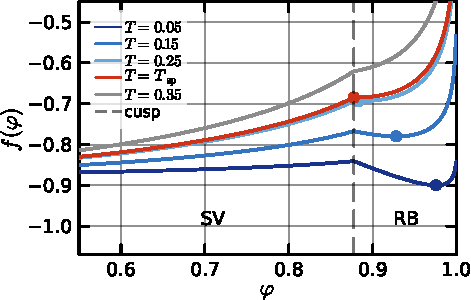
\includegraphics[width=0.45\textwidth]{panels_paper/cusp_illustration.pdf}
\caption{Leading-order free energy density $f(\varphi)$ at $\alpha=0.5$, $\Bnet=1$,
for several $T$. RB: retrieval basin; NRB: non-retrieval basin (where the
competitor sum dominates); cusp at $\varphi\approx 0.877$ (dashed grey).
Coloured dots mark the RB minima; they disappear at the spinodal temperature
$T_{\rm sp}(\alpha, \Bnet) \approx 0.262$.}
\label{fig:cusp}
\end{figure}

\paragraph{Stability and Kramers escape.}
For $T < T_{\mathrm{sp}}(\alpha, \Bnet)$ the retrieval minimum exists. It is
thermodynamically stable when it is the global minimum of $f$ and metastable when
the spurious-basin minimum is deeper. At equilibrium the deeper basin carries the
larger weight, with the ratio between the two basins set by their depth
difference; at finite $T$ and finite $N$ both basins can carry significant mass.
The chain escapes the retrieval basin to the spurious basin by a Kramers process
at the same rate $\sim \e^{-N \Delta f / T}$ in both
regimes~\citep{kramers1940, hanggi1990}, with $\Delta f$ the per-spin barrier from
the basin minimum to the cusp; what differs is the return rate. A Monte Carlo
ensemble initialised in the basin contains both populations at finite budget, in
proportions set by the budget over the Kramers escape time. As $T \to 0$ the
escape rate vanishes, so retrieval is retained whenever the basin exists.


% ----------------------------------------------------------------------------------
% ----------------------------------------------------------------------------------
% ----------------------------------------------------------------------------------
\section{Monte Carlo schemes}
\label{sec:mc}

The main issue of Monte Carlo simulations for validation of retrieval zones 
of the Dense Associative Memory with exponential capacity is the computational 
cost of evaluating the energy~\eqref{eq:lse} at each step, which involves 
a sum over $M = \e^{\alpha N}$ patterns. Thus, in addition to the standard 
Metropolis scheme that evaluates the full sum~\citep[e.g.,][]{iclr2026mc}, 
we introduce two approximations that reduce the cost per step, 
and we compare all three against the theoretical predictions. Below we assume $\Bnet = 1$.

\paragraph{Full.}
All $M = \lceil\e^{\alpha N}\rceil$ patterns are generated explicitly per
disorder realization and the log-sum is evaluated over all of them at
every step. Cost per step is $\mathcal{O}(MN)$, dominated by the dense 
$M \times N$ matrix-vector product that yields the $M$ pattern-state alignments;
we batch chains into a single matrix-matrix product to saturate the GPU. 
$M$ is fixed at the maximum the GPU memory allows, and $N$ is then
obtained from $N(\alpha) = \lceil \log M / \alpha \rceil$.  At each
$(\alpha, T)$ we draw 32 disorder realizations and follow two Metropolis
replicas per realization, both initialized at the target $\bxi^1$.  Step
size is $\sigma = 2.4\, T / \sqrt N$.  Each replica is equilibrated for
$N_{\rm eq} = 2^{15}$ steps and sampled for $N_{\rm samp} = 2^{13}$
steps.  Per cell we record the time-averaged target alignments
$\varphi_a, \varphi_b$ and the maximum non-target alignment.

\paragraph{Cone.}
This approximation is based on our finding that the spurious basin is formed
by the patterns near the saddle point. Thus, we introduce an alignment cutoff $\phi_{\mathrm{keep}}$ 
that partitions the pattern set into two pieces. Patterns with $\varphi_{1\mu} \geq \phi_{\mathrm{keep}}$
lie inside a spherical cone of half-angle $\arccos(\phi_{\mathrm{keep}})$
around the target $\bxi^1$; these are generated explicitly and enter the
log-sum term-by-term.  Patterns with $\varphi_{1\mu} < \phi_{\mathrm{keep}}$
make up the passive bulk and are absorbed into a single
$\bx$-independent constant
\begin{equation}
\ln C_{\mathrm{bulk}} = \alpha N + \ln \!\int_{-1}^{\phi_{\mathrm{keep}}}
 h(\phi)\,\e^{\Bnet N \phi}\,\dd\phi,
\label{eq:cbulk}
\end{equation}
which sits inside the log-sum on equal footing with the in-cone patterns.
The number of in-cone patterns per disorder is a Poisson draw with mean
$M\,p_{>}$, where $p_{>} = \Pr(\varphi \geq \phi_{\mathrm{keep}})$ under
the spherical density~\eqref{eq:exact_density}.  In the rescaled variable
$y = (1 + \phi)/2$, the spherical density becomes a symmetric Beta and
each in-cone pattern's alignment with $\bxi^1$ is drawn from the truncated
distribution
\begin{equation}
    y \sim \mathrm{Beta}\!\Bigl(\tfrac{N-1}{2}, \tfrac{N-1}{2}\Bigr)\,,
\label{eq:beta-tail}
\end{equation}
together with a uniform perpendicular direction on the $(N{-}2)$-sphere
orthogonal to $\bxi^1$.  The cone set is fixed once per disorder.
For our $\phi_{\rm keep}$ (see Results), the explicit pattern set
handled per step is smaller than $M$ by orders of magnitude; the rest
enters through the closed-form bulk integral.  Disorder count,
replicas, initial condition, step size, equilibration and sampling
lengths, and recorded observables are identical to Full.  We have
verified Cone-Full equivalence at a shared budget (see Results).

\paragraph{Bulk.}
No patterns are generated.  The chain evolves under the leading-order
analytical free energy of Section~\ref{sec:theory}, with retrieval
basin and spurious basin both produced by one closed-form profile
$f(\varphi)$.  Here $\phi^1 = \bxi^1 \cdot \bx /
N$~\eqref{eq:alignment} is the chain's alignment with the target.
The spurious sum is replaced by its disorder-averaged saddle
value~\eqref{eq:spurious_saddle},
$\e^{N(\alpha + \gmax(\Bnet) - \Bnet)}$, an $\bx$-independent
constant, and the softmax sum~\eqref{eq:softmax_sum} reduces to
two terms,
\begin{equation}
\ln S(\phi^1) = \ln\!\bigl[ \e^{\Bnet N (\phi^1 - 1)}
                + \e^{N (\alpha + \gmax(\Bnet) - \Bnet)} \bigr],
\label{eq:bulk-logS}
\end{equation}
at $\mathcal{O}(N)$ cost per step.

The Full and Cone rule $\sigma = 2.4\,T/\sqrt N$ shrinks as
$1/\sqrt N$, giving microscopic steps at Bulk's large-$N$ reach: at
$N = 10^4$ the chain cannot traverse the basin in
$T_{\mathrm{MC}} = 10^5$ steps, let alone resolve the Kramers escape
rate that sets the boundary.  We use the curvature-matched step
\begin{equation}
\gamma(\varphi) = f''(\varphi)
              = \frac{T\,(1 + \varphi^2)}{(1 - \varphi^2)^2},
\qquad
\sigma^2 = \frac{2 T}{\gamma(\varphi_{\rm eq})}
       = \frac{2\,(1 - \varphi_{\rm eq}^2)^2}{1 + \varphi_{\rm eq}^2},
\label{eq:bulk-sigma}
\end{equation}
where $\gamma(\varphi)$ is the second derivative of the leading-order
free energy density $f$ and $\gamma_{\rm eq} \equiv \gamma(\varphi_{\rm eq})$
is its value at the basin minimum.  The explicit $T$ in $\sigma$
cancels against $T$ in $\gamma$; the only remaining dependence is
through $\varphi_{\rm eq}(T)$, and $\sigma$ is $N$-independent.
$\gamma(\varphi)$ diverges at the sphere edge $\varphi = \pm 1$, so
the curvature-matched step $\sqrt{2T/\gamma(\varphi)}$ vanishes
there: a chain at $\phi^1 = 1$ has no admissible step under this
rule.  We therefore initialize at the basin minimum,
$\phi^1 = \varphi_{\rm eq}(T)$~\eqref{eq:phi_eq}, with perpendicular
components uniform on the sphere of radius
$\sqrt N \,\sqrt{1 - \varphi_{\rm eq}^2}$; there $\gamma$ is finite,
$\sigma$ is curvature-matched by construction, and acceptance is
$\approx 0.37$ at every $N$.

We run Bulk at $N \in \{100, 300, 10^4\}$.  Per $\alpha$ we scan $T$
downward from $\min(T_{\rm sp}(\alpha), 0.495)$ in steps of $0.01$,
running $64$ independent chains of $T_{\mathrm{MC}} = 10^5$ steps each,
and record $T_{\rm bd}(\alpha)$ as the largest $T$ at which the
residual $\varphi_{\rm eq}(T) - \avg{\phi^1}$ first stays below $0.02$
for three consecutive $T$-steps.  There is no disorder.

\paragraph{What each scheme tests.}
The three schemes validate different things.  Full uses all $M$
patterns explicitly and serves as the ground-truth reference; the
only approximation is Monte Carlo noise.  Cone drops the patterns
with $\varphi_{1\mu} < \phi_{\rm keep}$ (almost all of $M$, with
near-zero alignment to the target) and replaces them by a single
constant from the analytical bulk integral~\eqref{eq:cbulk}; Cone
matching Full at a shared $M$ validates this analytical bulk
integral to within MC noise.  Bulk drops all patterns and uses the
leading-order value $\gmax(\Bnet)$ in $\ln S$~\eqref{eq:bulk-logS}.
It runs at $\mathcal{O}(N)$ cost per step and reaches $N$ much
larger than Full or Cone can; the convergence of its boundary to the
spinodal as $N$ grows validates the leading-order Kramers picture in
the asymptotic limit.


% ----------------------------------------------------------------------------------
% ----------------------------------------------------------------------------------
% ----------------------------------------------------------------------------------

\section{Results}
\label{sec:results}

A single NVIDIA RTX A6000 GPU card with 50 Gb memory allows 
$M = 4.4 \times 10^6$ patterns for the Full scheme (\texttt{Float32}), resulting in
$N(\alpha) = \lceil \log M / \alpha \rceil$ from $N = 76$ at
$\alpha = 0.20$ to $N = 24$ at $\alpha = 0.65$, with a full
$(\alpha, T)$ sweep taking about $26$ days.  Cone scheme at
$M = 3.0 \times 10^8$ with $\phi_{\rm keep} = 0.40$ keeps the typical
in-cone count $K$ below $1.3\%$ of $M$ at every cell, resulting in $N$ from
$98$ to $30$ over the same $\alpha$ range, and sweep taking in about $7$ days.  Bulk
has no patterns and runs at $\mathcal{O}(N)$ per step on a 16-thread
CPU, reaching $N \in \{100, 300, 10^4\}$ in about one, five, and
ninety minutes per sweep.  We verified Cone-Full equivalence at
the shared budget $M = 4.4 \times 10^6$.

Fig.~\ref{fig:heatmap} shows the $(\alpha, T)$ stability diagram at
$\Bnet = 1$, from the Cone Monte Carlo sampler at two budgets,
$M = 4.4 \times 10^6$ and $M = 3.0 \times 10^8$. The heatmap encodes the
residual $\varphi_{\mathrm{eq}}(T) - \langle\varphi\rangle$ from the
$M = 3.0 \times 10^8$ run: white where the chain remains in the retrieval
basin, red where it escapes to the spurious basin. The blue staircases trace,
for each $\alpha$ column, the lowest $T$ at which roughly 5\% of chain
endpoints have escaped from the retrieval basin to the spurious basin.
Operationally, this is the threshold
$\varphi_{\mathrm{eq}}(T) - \langle\varphi\rangle > 0.02$ at the
basin-to-saddle gap $\Delta\varphi \approx 0.40$ along the boundary, after
a light smoothing pass to suppress single-cell MC noise. At fixed $\alpha$, 
increasing the budget from $M = 4.4 \times 10^6$ to
$M = 3.0 \times 10^8$ (which raises the reachable $N$ via the $N$-ramp)
shifts the boundary to higher $T$. The expected destination at
$N \to \infty$ is the spinodal $T_{\rm sp}(\alpha, \Bnet)$~\eqref{eq:spinodal}:
below the spinodal the retrieval basin still exists, and a chain initialised
in the basin escapes only on the Kramers time
$\tau_K \sim \e^{N \Delta f / T}$, which grows exponentially with $N$.  At
the $N$ values reached by the Cone sampler here ($N \le 98$) the boundary
is still far from the spinodal.  It lies close to the saddle
line $\acSd(\Bnet, T)$~\eqref{eq:capacity_T}, but this proximity is
incidental: as established in Section~\ref{sec:theory}, $\acSd$ is a
thermodynamic crossover, not a sharp boundary, with no sharp change
in the retrieval fraction as we cross it.  The Gaussian prediction
$\acGauss(T)$ sits to the left of both Cone boundaries, underestimating
the capacity at every $T$.

\paragraph{Finite-$N$ residual basin near the LSE tip.}
At low $T$ near the tip $\ac(\Bnet,0) = \Bnet - \gmax(\Bnet) = 0.6226$
at $\Bnet=1$ the Cone boundary in Fig.~\ref{fig:heatmap} sits to the
right of the LO spinodal, reaching $\alpha \approx 0.70$ at
$T = 0.005$.  The deviation is a smoothing effect.  The
softmax sum~\eqref{eq:softmax_sum}, with the spurious term replaced
by its Laplace value~\eqref{eq:spurious_laplace} from Appendix~A,
defines the finite-$N$ effective potential
\begin{multline}
\frac{V_N(\phi)}{N} = 1 - \tfrac{1}{\Bnet N}\,
   \ln\!\Big[\e^{\Bnet N \phi} +\\
            \frac{\e^{\Bnet N \varphi_c(\alpha, \Bnet)}}{(1-\varphi^{*4}(\Bnet))^{1/2}} \Big]
    - \tfrac{T(N-3)}{2N}\,\ln(1 - \phi^{2}),
\label{eq:V-finite-N}
\end{multline}
whose $N \to \infty$ limit is the LO landscape
$1 - \max(\phi, \varphi_c) - (T/2)\ln(1 - \phi^2)$.  At finite $N$
the log-sum smooths the LO corner over width $(\Bnet N)^{-1}$.
Whenever $\varphi_c$ sits just above $1$ that smoothing reaches onto
the sphere and produces a local minimum of $V_N$ at $\phi$ slightly
below $1$ that the LO curve does not have.
Fig.~\ref{fig:Veff_finite_N} shows the three landscapes at
$\alpha = 0.62, 0.65, 0.70$, $T = 0.005$, for the $N(\alpha)$ that
the $M = 4.4 \times 10^6$ Cone run reaches.  The $V_N$ minimum from
$V_N'(\phi)=0$ sits at $\phi = 0.995, 0.992, 0.977$; the Cone
$\langle\phi\rangle$ at the same cells is $0.995, 0.991, 0.975$ —
within $0.002$ at every load.  As $N$ grows the smoothing width
$1/(\Bnet N)$ shrinks, the residual minimum retreats toward
$\phi=1$, and the deviation past the LO tip closes — visible
across the Bulk curves in Fig.~\ref{fig:heatmap}, where the
$N = 10^4$ boundary lies on top of the LO spinodal at this $T$.

The green curves trace the Bulk boundary at the same threshold,
$T_{\mathrm{MC}} = 10^5$ steps per chain, and
$N \in \{100,\, 300,\, 10^4\}$.  Bulk carries no live patterns ($K = 0$)
and the chain follows the two-term log-sum~\eqref{eq:bulk-logS} directly,
so the line is the pure Kramers-escape boundary from the basin minimum
at finite $N$.  Empirically the gap to the spinodal shrinks as
$1/\sqrt N$: at $\alpha = 0.50$ the gap drops from $\Delta T \approx
0.13$ at $N = 100$ to $0.08$ at $N = 300$, and by $N = 10^4$ the
boundary sits within one $T$-grid cell of the spinodal across
$\alpha \in [0.40,\, 0.62]$ and is visually indistinguishable from it
(the spinodal in the figure is drawn last, on top of the lightest green
$N = 10^4$ curve, by design).  The march of the Bulk boundary onto the
spinodal as $N$ grows is the asymptotic claim the theory makes, now
visible across two decades of $N$ in a single figure.

Dependence of the Bulk boundary on the MC budget is much weaker than on
$N$.  Solving the 5\% criterion $T_{\mathrm{MC}}\,k = 0.05$ for the
Kramers rate $k = (1/2\pi)\,\e^{-N\Delta f / T}$ gives
$N\Delta f / T = \ln T_{\mathrm{MC}} + O(1)$, so the gap to the spinodal
grows only as $\sqrt{\ln T_{\mathrm{MC}}}$: about 9\% per decade in
$T_{\mathrm{MC}}$ from the present $T_{\mathrm{MC}} = 10^5$, against the
$\sqrt{10} \approx 3.16$ shrinkage per decade in $N$.  Concretely, going
from $T_{\mathrm{MC}} = 10^5$ to $10^6$ would shift the $N = 100$ Bulk
line by $\Delta T_{\mathrm{bd}} \approx 0.01$--$0.04$ at $T \ge 0.2$ and
by less than the $T$-grid spacing $\dd T = 0.01$ at $T \le 0.05$.  Near
the LSE capacity tip $\alpha_{\rm LSE} \approx 0.6226$ the spinodal
itself collapses to $T_{\mathrm{sp}} = 0$, so the absolute gap budget is
small and $T_{\mathrm{MC}}$ shifts there are pinned below the $T$-grid
spacing.  Convergence to the spinodal in the figure is therefore
controlled by $N$; multiplying the per-chain budget by orders of
magnitude would barely move any of the three green curves.

\begin{figure*}[t]
\centering
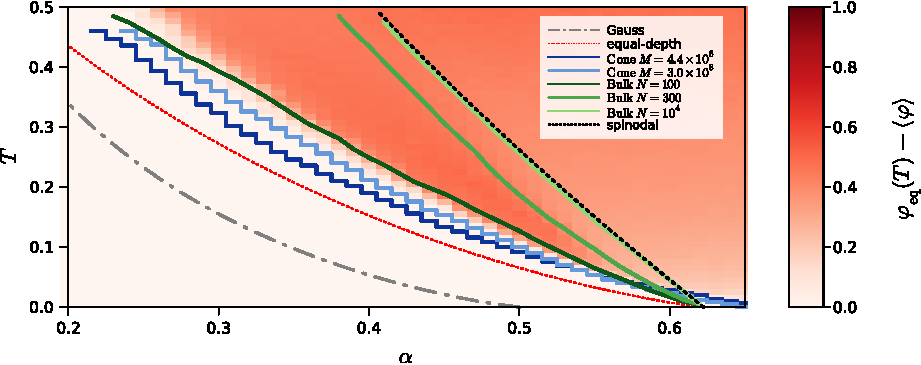
\includegraphics[width=0.9\textwidth]{panels_paper/heatmap_textwidth_profile.pdf}
\caption{$(\alpha, T)$ stability diagram at $\Bnet = 1$. Heatmap:
$\varphi_{\mathrm{eq}}(T) - \langle\varphi\rangle$ from the
$M = 3.0 \times 10^8$ Cone MC run.  Blue staircases: Cone retrieval
boundary at threshold $0.02$ (roughly 5\% of chain endpoints escaped) for
$M = 4.4 \times 10^6$ (dark) and $M = 3.0 \times 10^8$ (light).  Green
curves: Bulk retrieval boundary at $T_{\mathrm{MC}} = 10^5$ and
$N \in \{100,\, 300,\, 10^4\}$, dark to light with $N$.  The light-green
$N = 10^4$ curve sits on the spinodal across most of the $\alpha$ range;
the spinodal is drawn last to make this coincidence visible.  Reference curves:
saddle boundary $\acSd(\Bnet, T)$~\eqref{eq:capacity_T} (red dotted),
spinodal $T_{\mathrm{sp}}$~\eqref{eq:spinodal} (black dotted), Gaussian
baseline $\acGauss(T)$ (grey dash-dotted).}
\label{fig:heatmap}
\end{figure*}

\begin{figure*}[t]
\centering
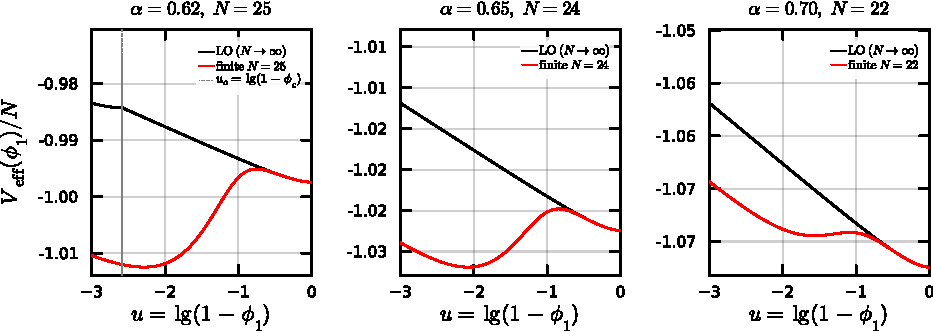
\includegraphics[width=0.9\textwidth]{panels_paper/Veff_finite_N.pdf}
\caption{Finite-$N$ effective potential $V_N(\phi)/N$ at
$\Bnet = 1$, $T = 0.005$, against $\phi$ on a $\lg(1-\phi)$ axis for
three loads above $\ac(\Bnet, 0) = 0.6226$.  Black: leading-order
landscape $-\max(\phi, \varphi_c) - (T/2)\log(1-\phi^2)$.
Red: the finite-$N$ form~\eqref{eq:V-finite-N} at $N(\alpha)$ for
the Cone run at $M = 4.4 \times 10^6$.  The log-sum smooths the LO
corner over width $\sim 1/(\Bnet N)$, generating a local minimum
near $\phi = 1$ that the LO curve lacks.  Red dots: $V_N$
residual-basin minima.  Black dot (left panel only): LO
retrieval-basin minimum at $\phi = \varphi_{\rm eq}(T)$, present only
when $\varphi_c < 1$.  Grey dotted: LO cusp position $\varphi_c$,
shown only when $\varphi_c < 1$.}
\label{fig:Veff_finite_N}
\end{figure*}


% ----------------------------------------------------------------------------------
% ----------------------------------------------------------------------------------
% ----------------------------------------------------------------------------------

\section{Discussion}
\label{sec:discussion}






% ----------------------------------------------------------------------------------
% ----------------------------------------------------------------------------------
% ----------------------------------------------------------------------------------

% \section{Acknowledgments}


\bibliography{aaai2026}

\appendix

\section{Appendix A: Derivation of the prefactor in the spurious sum}

The integral~\eqref{eq:spur_integral} evaluates in closed form. Substituting
$\varphi = \cos\theta$ maps the spherical density onto the kernel of the integral
representation of the modified Bessel function
$I_\nu(z)$~\citep[8.431.3]{gradshteyn2015}; at $\nu = N/2 - 1$, $z = \Bnet N$,
this gives for $N > 1$
\begin{equation}
S_{\rm spur} = M \Gamma\Big(\tfrac{N}{2}\Big)\left(\frac{2}{\Bnet N}\right)^{\!N/2-1}\!\!\e^{-\Bnet N}\,I_{N/2-1}(\Bnet N).
\label{eq:spurious_exact}
\end{equation}
The right-hand side is the disorder expectation of the sum~\eqref{eq:spur_sum}. The
relative fluctuations of $S_{\rm spur}$ around this expectation are
$\sim \e^{N[\delta(\Bnet) - \alpha]/2}$ with
$\delta(\Bnet) = g_{\max}(2\Bnet) - 2\,g_{\max}(\Bnet) > 0$; they are exponentially
small in $N$ when $\alpha > \delta(\Bnet)$. At $\Bnet = 1$, $\delta \approx 0.334$,
well below the retrieval boundary $\alpha_c \approx 0.623$, so the
saddle~\eqref{eq:spurious_saddle} captures the typical $S_{\rm spur}$.


The Debye uniform asymptotic of the modified Bessel function~\citep[10.41.3]{olver2010nist}
gives the prefactor of~\eqref{eq:spurious_saddle}. Keeping the leading ($k = 0$) term of
the asymptotic series,
\begin{equation}
I_\nu(\nu z') \sim \frac{\e^{\nu\eta(z')}}{(2\pi\nu)^{1/2}(1+{z'}^2)^{1/4}},
\end{equation}
where $z' = 2\Bnet N/(N-2)$ and
\begin{equation}
    \eta(z') = \sqrt{1+{z'}^2} + \ln\frac{z'}{1+\sqrt{1+{z'}^2}}\,.
    \label{eq:bessel_debye}
\end{equation}  
$\eta(z')$ is expanded to $\mathcal{O}(N^{-1})$ because it is multiplied by
$\nu = N/2 - 1$ in the exponent:
\begin{equation}
    \eta(z') = \eta(2\Bnet) + \eta'(2\Bnet) \frac{4\Bnet}{N} + O(N^{-2})\,,
\end{equation}
where
\begin{align}
    \eta(2\Bnet)  &= 1 + 2\Bnet\varphi^* + \ln\varphi^*\,, \\
    \eta'(2\Bnet) &= \varphi^* + \frac{1}{2\Bnet}\,.
\end{align}
Then 
\begin{equation}
    \nu \eta(z') = \tfrac{N}{2} \eta(2\Bnet) - \ln\varphi^* + \mathcal{O}(1/N).
\end{equation}
The $\mathcal{O}(1)$ piece $-\ln\varphi^*$ in the exponent contributes a factor
$1/\varphi^*$ to the prefactor. Using Stirling's formula
\begin{equation}
    \Gamma(N/2) \sim \sqrt{4\pi/N}\,(N/2)^{N/2}\,\e^{-N/2}
\end{equation} 
and collecting all terms in~\eqref{eq:spurious_exact} to $\mathcal{O}(1)$ in the
exponent and to leading order in the prefactor reproduces the exponent
of~\eqref{eq:spurious_saddle} and gives the prefactor:
\begin{equation}
S_{\rm spur} \approx \frac{\e^{N[\alpha + g_{\max}(\Bnet) - \Bnet]}}{\sqrt{1-\varphi^{*4}}}
\label{eq:spurious_laplace}
\end{equation}
with $g_{\max}(\Bnet)$ given by \eqref{eq:saddle_value}.
At $\Bnet = 1$, $\varphi^* \approx 0.618$ and the prefactor is $\approx 1.082$.


\section{Appendix B: Tangency of the cusp lines to the spherical extreme}

To show that the cusp lines \eqref{eq:cusp} are tangent to the
spherical-extreme curve \eqref{eq:varphi_max} at every
$\Bnet$, we need to show that the slope and the $\varphi$-intercept
coincide.

Differentiating \eqref{eq:varphi_max} once gives
\begin{equation}
\varphi_{\max}'(\alpha) \;=\; \frac{1-\varphi_{\max}^2}{\varphi_{\max}},
\label{eq:tangent_slope_C}
\end{equation}
and a second differentiation gives $\varphi_{\max}''(\alpha) < 0$ for $\alpha > 0$,
so $\varphi_{\max}$ is strictly concave on $(0, \infty)$. For a concave function
every tangent line lies above the function, with equality only at the tangency
point. This is used in the lower-envelope identity below.

The cusp line at sharpness $\Bnet$,
\begin{equation}
\varphi \;=\; \alpha/\Bnet + g_{\max}(\Bnet)/\Bnet,
\end{equation}
has slope $1/\Bnet$ and $\varphi$-intercept $g_{\max}(\Bnet)/\Bnet$. To find the point on
the blue curve where the tangent has the same slope, set the right-hand side
of~\eqref{eq:tangent_slope_C} equal to $1/\Bnet$:
\begin{equation}
\frac{1-\varphi^2}{\varphi} \;=\; \frac{1}{\Bnet}
\quad\Longleftrightarrow\quad
\Bnet\,\varphi^2 + \varphi - \Bnet = 0.
\label{eq:saddle_eq_C}
\end{equation}
This is the saddle equation and its unique positive root is the spherical saddle \eqref{eq:saddle}.
The corresponding $\alpha$ on the blue curve follows from
$\varphi^* = \varphi_{\max}(\alpha^*)$:
\begin{equation}
\alpha^*(\Bnet) \;=\; -\tfrac12 \ln(1-\varphi^{*\,2}).
\label{eq:alpha_star_C}
\end{equation}

A line of slope $1/\Bnet$ passing through $(\alpha^*(\Bnet), \varphi^*(\Bnet))$ has
$\varphi$-intercept
\begin{equation}
b_{\rm tg}(\Bnet) \;=\; \varphi^* - \alpha^*/\Bnet.
\end{equation}
The cusp line has $\varphi$-intercept $g_{\max}(\Bnet)/\Bnet$.
Using~\eqref{eq:saddle_value}, the $\varphi$-intercepts coincide;
the two lines are therefore identical.

By the concavity statement above, the cusp line at any sharpness $\Bnet$ lies above the blue curve, with equality only at
$\alpha = \alpha^*(\Bnet)$:
\begin{equation}
\varphi_c(\alpha, \Bnet) \;\ge\; \varphi_{\max}(\alpha) \quad \text{for all $\alpha$ and all $\Bnet > 0$},
\end{equation}
with equality at one $\alpha$ for each $\Bnet$. Taking the infimum over $\Bnet$,
\begin{equation}
\varphi_{\max}(\alpha) \;=\; \inf_{\Bnet > 0} \varphi_c(\alpha, \Bnet),
\label{eq:lower_envelope_C}
\end{equation}
the lower-envelope identity.

The saddle function $\varphi^*(\Bnet)$~\eqref{eq:saddle} is
continuous and strictly increasing on $(0, \infty)$ from $0$ to $1$. As $\Bnet$ sweeps $(0, \infty)$,
the tangency point $(\alpha^*(\Bnet), \varphi^*(\Bnet))$ therefore traces the
entire blue curve from the origin to its right edge.

Two results follow from the geometric setup above.  At $T = 0$ the
cusp line of slope $1/\Bnet$ reaches $\varphi = 1$ at
$\alpha = \Bnet - g_{\max}(\Bnet)$, which is the zero-temperature
capacity~\eqref{eq:capacity_T0} (equivalently, the spinodal at
$T = 0$).

\textbf{Ramsauer's bound is too restrictive.}  The \citeauthor{ramsauer2021hopfield}'s condition
$\varphi_{\max}(\alpha) = 1 - \alpha/\Bnet$ is the intersection of
$\varphi_{\max}$ with the line of slope $-1/\Bnet$ through $(0, 1)$.
By~\eqref{eq:lower_envelope_C}, $\varphi_{\max}$ lies below every
cusp line, so the \citeauthor{ramsauer2021hopfield}'s line crosses $\varphi_{\max}$ at strictly
smaller $\alpha$ than the cusp line at slope $1/\Bnet$ reaches
$\varphi = 1$.  \citeauthor{ramsauer2021hopfield}'s capacity $\alpha_c^R$ therefore satisfies
$\alpha_c^R < \alpha_c(\Bnet, 0)$ for every $\Bnet > 0$.

\textbf{Asymptotic capacity.}  Using \eqref{eq:saddle} in
\eqref{eq:saddle_value} and then in \eqref{eq:capacity_T0}, one obtains:
\begin{equation}
\begin{aligned}
\ac(\Bnet, 0) = \Bnet - g_{\max}(\Bnet) &\;\to\; \Bnet
   && (\Bnet \to 0),\\
\ac(\Bnet, 0) = \Bnet - g_{\max}(\Bnet) &\;\to\; \tfrac{1}{2}\ln\Bnet + \tfrac{1}{2}
   && (\Bnet \to \infty),
\end{aligned}
\label{eq:asymptotic_C}
\end{equation}
the small- and large-$\Bnet$ limits of the zero-temperature capacity
cited in the Abstract.

\paragraph{Legendre transform.}
The lower-envelope identity~\eqref{eq:lower_envelope_C} and the formula
below are the two sides of a Legendre transform between
$\varphi_{\max}(\alpha)$ and $g_{\max}(\Bnet)/\Bnet$.  The forward
transform takes $\varphi_{\max}$ to its conjugate,
\begin{equation}
g_{\max}(\Bnet)/\Bnet \;=\; \sup_\alpha\,\bigl[\,\varphi_{\max}(\alpha) - \alpha/\Bnet\,\bigr],
\label{eq:legendre_C}
\end{equation}
with the supremum attained at $\alpha = \alpha^*(\Bnet)$ from the
slope-match condition~\eqref{eq:saddle_eq_C}.  The Legendre transform
is involutive: applying it to $g_{\max}(\Bnet)/\Bnet$ recovers
$\varphi_{\max}(\alpha)$, which is exactly~\eqref{eq:lower_envelope_C}
after using the cusp-line definition~\eqref{eq:cusp}.

Two facts follow from the duality.  First, the lower-envelope
identity~\eqref{eq:lower_envelope_C} is the inverse
of~\eqref{eq:legendre_C}, so the tangency is automatic.  Second,
differentiating~\eqref{eq:saddle_value} in $\Bnet$ and using the
envelope theorem $\p g/\p\varphi|_{\varphi^*} = 0$ gives
\begin{equation}
g_{\max}'(\Bnet) \;=\; \varphi^*(\Bnet),
\label{eq:envelope_C}
\end{equation}
so $g_{\max}(\Bnet)$ is recovered by integrating $\varphi^*(\Bnet)$.
Plugging the small- and large-$\Bnet$ limits $\varphi^* \sim \Bnet$
and $\varphi^* \sim 1 - 1/(2\Bnet)$ into~\eqref{eq:envelope_C} and
integrating reproduces~\eqref{eq:asymptotic_C}.


\section{Appendix C: Translation of \citeauthor{ramsauer2021hopfield}'s storage-capacity bound}
\label{sec:appendix_ramsauer}

We give a literal symbol-by-symbol map between
\citeauthor{ramsauer2021hopfield}'s notation and ours, then derive
the Theorem~4 reading, Eq.~\eqref{eq:ramsauer_bound} and
Eq.~\eqref{eq:ramsauer_capacity} step by step.

\paragraph{Notation map.}
\citeauthor{ramsauer2021hopfield} use $N$ patterns
$\bm x_i \in \mathbb R^d$ on a sphere of radius
$\mathbf M := K\sqrt{d-1}$ with sharpness $\beta$, and a query
$\bm \xi \in \mathbb R^d$.  Our patterns are
$\bxi^\mu \in \mathbb R^N$, $\mu = 1, \dots, M$, on a sphere of
radius $\sqrt N$ with sharpness $\Bnet$; the target is $\bxi^1$ and
the query is taken at the target.  Setting $K = 1$ in
\citeauthor{ramsauer2021hopfield}'s convention identifies the
pattern norm $\mathbf M = \sqrt{d-1}$ with our $\sqrt N$ in the
large-$N$ limit.  The variable map is
\begin{center}
\begin{tabular}{lll}
\hline
\citeauthor{ramsauer2021hopfield} & here & meaning \\
\hline
$N$ & $M = \e^{\alpha N}$ & number of patterns \\
$d$ & $N$ & pattern dimension \\
$\mathbf M$ & $\sqrt N$ & pattern norm \\
$\beta$ & $\Bnet$ & softmax sharpness \\
$\bm x_i^\top \bm x_j$ & $N\,\varphi^{ij}$ & pair product \\
$\bm x_i$, $\bm \xi$ & $\bxi^i$, $\bxi^1$ & patterns, target query \\
\hline
\end{tabular}
\end{center}
With the query at the target, $\bm \xi^\top \bm x_1 = N$ and
$\bm \xi^\top \bm x_j = N\,\varphi^{1j}$ for $j \geq 2$.  The
\emph{maximum competitor alignment} is
$\varphi_{\max} = \max_{j \neq 1}\varphi^{1j}$.

\paragraph{Theorem~4 reading: retrieval ties to $N(1-\varphi_{\max})$.}
The separation, their Eq.~(5), is
\begin{equation*}
\Delta_i \;:=\; \bm x_i^\top \bm x_i - \max_{j \neq i}\bm x_i^\top \bm x_j.
\end{equation*}
At the target $i = 1$ we substitute the map: $\bm x_1^\top \bm x_1 = N$
and $\max_{j \neq 1}\bm x_1^\top \bm x_j = N\,\varphi_{\max}$.  Hence
\begin{equation*}
\Delta_1 \;=\; N\,(1 - \varphi_{\max}).
\end{equation*}
Their Theorem~5, Eq.~(9), bounds the retrieval error of pattern
$\bm x_1$ by
\begin{equation*}
\|\bm x_1 - \bm x_1^*\| \;\leq\; 2 e\,(N-1)\,\mathbf M\,\e^{-\beta \Delta_1}.
\end{equation*}
Substituting the map ($N \to M$, $\mathbf M \to \sqrt N$,
$\beta \to \Bnet$, $\Delta_1 \to N(1-\varphi_{\max})$):
\begin{equation*}
\|\bxi^1 - \bxi^{1*}\| \;\leq\; 2 e\,M\,\sqrt N\,\e^{-\Bnet N(1-\varphi_{\max})}.
\end{equation*}
For this bound to guarantee retrieval (error below any fixed
$\epsilon$ at large $N$) we need the exponential to overcome the
prefactor, i.e.
\begin{equation*}
\Bnet N (1-\varphi_{\max}) \;>\; \ln M + O(\ln N) \;=\; \alpha N + O(\ln N),
\end{equation*}
since $M = \e^{\alpha N}$.  To leading order in $N$ this is
$\varphi_{\max} < 1 - \alpha/\Bnet$.  As $\varphi_{\max} \to 1$ the
exponential factor approaches $1$, the bound no longer guarantees
small retrieval error, and Theorem~4 stops securing retrieval.  In
this sense Theorem~4 ties retrieval to the separation
$N(1-\varphi_{\max})$, and retrieval fails when
$\varphi_{\max} \to 1$.

\paragraph{Derivation of Eq.~\eqref{eq:ramsauer_bound}.}
The shifted spurious sum~\eqref{eq:spur_sum} is
\begin{equation*}
S_{\rm spur} \;=\; \sum_{\mu = 2}^M \e^{\Bnet N (\varphi^\mu - 1)}.
\end{equation*}
For every $\mu \geq 2$, $\varphi^\mu \leq \varphi_{\max}$ by
definition of $\varphi_{\max}$, so
\begin{equation*}
\e^{\Bnet N (\varphi^\mu - 1)} \;\leq\; \e^{\Bnet N (\varphi_{\max} - 1)}
   \;=\; \e^{-\Bnet N (1-\varphi_{\max})}.
\end{equation*}
The sum of $M - 1$ terms, each at most this maximum, satisfies
\begin{equation*}
S_{\rm spur} \;\leq\; (M-1)\,\e^{-\Bnet N (1-\varphi_{\max})}
   \;\leq\; M\,\e^{-\Bnet N (1-\varphi_{\max})}.
\end{equation*}
Using $M = \e^{\alpha N}$ on the right,
\begin{equation*}
M\,\e^{-\Bnet N (1-\varphi_{\max})}
   \;=\; \e^{\alpha N - \Bnet N (1-\varphi_{\max})}
   \;=\; \e^{N(\alpha - \Bnet(1-\varphi_{\max}))},
\end{equation*}
which is Eq.~\eqref{eq:ramsauer_bound}.  The $M$-times-largest step
is the same one \citeauthor{ramsauer2021hopfield} use in their
Lemma~A4 Eq.~(134) for the softmax probability mass on competitors;
applying it to the unnormalised shifted sum gives the bound on
$S_{\rm spur}$ above.

\paragraph{Derivation of Eq.~\eqref{eq:ramsauer_capacity}.}
The shifted softmax sum~\eqref{eq:softmax_sum} reads
$S(\bm x) = 1 + S_{\rm spur}$ at the target, since the retrieval
term equals $\e^{\Bnet N(\varphi^1 - 1)} = 1$ for $\varphi^1 = 1$.
Retrieval requires the retrieval term to dominate, $S_{\rm spur} < 1$;
substituting the bound just derived,
\begin{equation*}
S_{\rm spur} < 1 \quad\Longleftarrow\quad
\e^{N(\alpha - \Bnet(1-\varphi_{\max}))} < 1
\quad\Longleftrightarrow\quad
\alpha < \Bnet\,(1-\varphi_{\max}),
\end{equation*}
or $\varphi_{\max} < 1 - \alpha/\Bnet$, the same threshold as in the
Theorem~4 reading.  The capacity is where this inequality saturates,
$\varphi_{\max}(\alpha) = 1 - \alpha/\Bnet$.  Substituting the
exact-density extreme alignment~\eqref{eq:varphi_max},
$\varphi_{\max}(\alpha) = \sqrt{1 - \e^{-2\alpha}}$,
\begin{equation*}
\sqrt{1 - \e^{-2\alpha}} \;=\; 1 - \frac{\alpha}{\Bnet},
\end{equation*}
which is Eq.~\eqref{eq:ramsauer_capacity}.  The Gaussian alternative
$\varphi_{\max}(\alpha) = \sqrt{2\alpha}$, used in
\citet{icml2026theory}, instead gives
$\sqrt{2\alpha} = 1 - \alpha/\Bnet$; at $\Bnet \to \infty$ this
reduces to $\acGauss = 1/2$.

\end{document}
